\chapter{Instalación de la Interfaz}
\label{apendiceB}
\lhead{Apéndice B.}

\section{Instalaciones en el OpenROV}

Esta interfaz fue probada en la versión de la imagen flash 30.0.3.

\subsection{Conexión SSH}

Para realizar las instalaciones necesarias en el OpenROV, este debe estar conectado a internet, por lo que es necesario implementar la siguiente configuración:
\begin{enumerate}
    \item Conectar el BBB directamente a un router usando un cable de ethernet.
    \item Conectar el BBB a la computadora usando un cable USB-miniUSB.
    \item Configurar el puerto de USB de la computadora con la IP 192.168.7.1(\textit{gateway} de la interfaz usb0. Ver \ref{tab:usb0eth0}) y máscara de red: 255.255.255.0.
    \item SSH al BBB con: \verb|ssh rov@192.168.7.2| \ref{tab:UserPass}
    \item Abrir Cockpit en el navegador en la dirección 192.168.254.1.
    \item Conectar el BBB a internet con el interfaz eth0 siguiendo las indicaciones del Apéndice A (A.2.2.2).
    \item Modificar el \verb|source.list| como se explica en el Apéndice A (A.2.4.2)
    \item Se desactiva el proxy: \verb|$ sudo /etc/init.d/openrov-proxy stop|
    
        \begin{figure}[H]
            \centering
            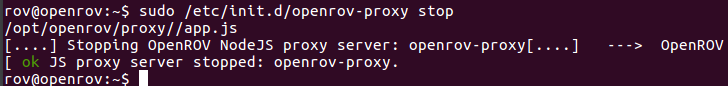
\includegraphics[scale=0.70]{partes/ImgSophia/ApendiceB/detenerproxy.png}
            \caption{Detener el proxy}
            \label{fig:StopProxy}
        \end{figure}
\end{enumerate}

\subsection{Descarga de dependencias}
\begin{verbatim}
$ sudo apt-get update
$ sudo apt-get install g++ libcairo2-dev libjpeg62-turbo-dev 
libpango1.0-dev libgif-dev build-essential 
\end{verbatim}

\subsubsection{Instalación de canvas}
\begin{verbatim}
$ sudo chown -R $USER /usr/local
$ cd /opt/openrov/cockpit/src/plugins
$ npm install canvas@1.2.2    
\end{verbatim}

Si se presentan errores durante la instalación como se muestra en la figura \ref{fig:ErrorCanvas} 

        \begin{figure}[H]
            \centering
            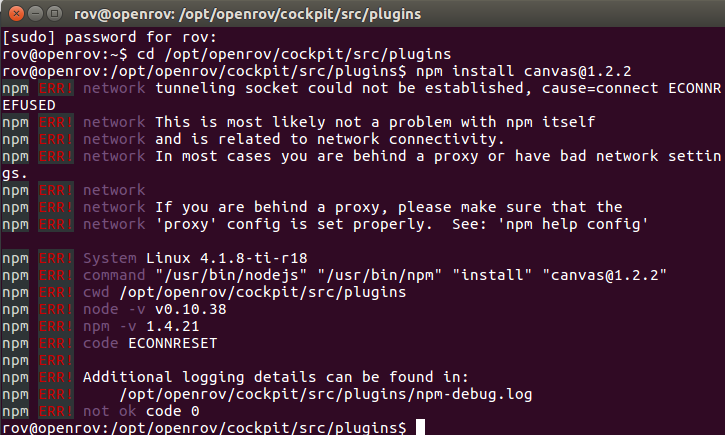
\includegraphics[scale=0.60]{partes/ImgSophia/ApendiceB/errorInstalandoCanvas.png}
            \caption{Error instalando canvas}
            \label{fig:ErrorCanvas}
        \end{figure}

Probar detendiendo el proxy o cerrando el terminal e iniciando una nueva sesión, y volver a intentar:
\begin{verbatim}
$ cd /opt/openrov/cockpit/src/plugins
$ npm install canvas@1.2.2    
\end{verbatim}

        \begin{figure}[H]
            \centering
            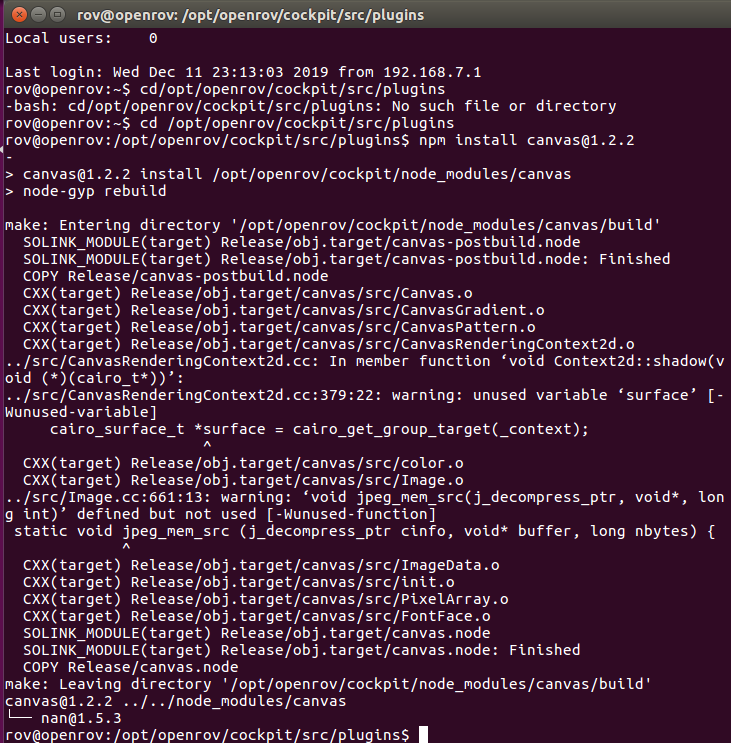
\includegraphics[scale=0.70]{partes/ImgSophia/ApendiceB/instalacionCanvasCompleta.png}
            \caption{Resultado de la instalación de canvas}
            \label{fig:InsCanvas}
        \end{figure}

\subsubsection{Instalación roslib}
\begin{verbatim}
$ npm install roslib@0.15.0    
\end{verbatim}

        \begin{figure}[H]
            \centering
            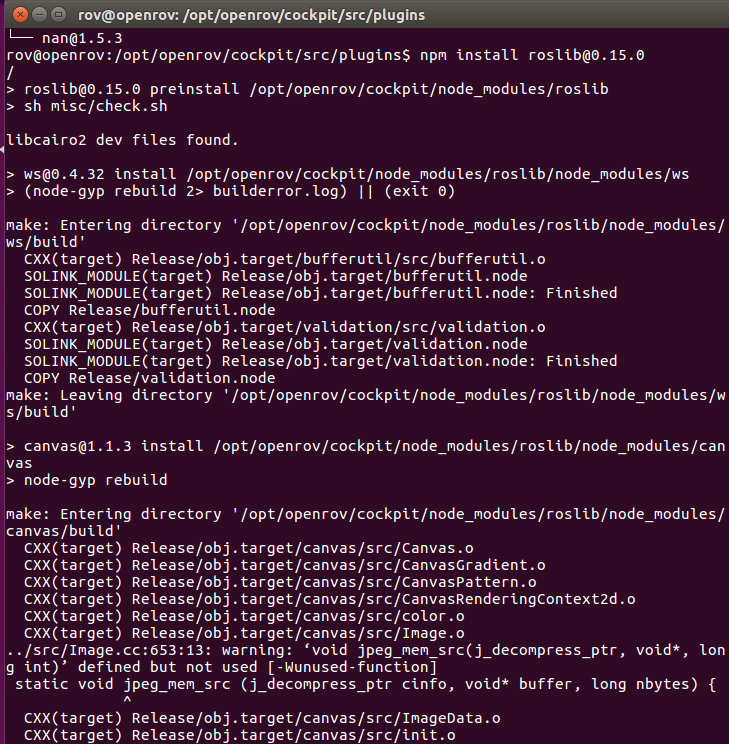
\includegraphics[scale=0.70]{partes/ImgSophia/ApendiceB/instalacionRoslib1.png}
            \caption{Inicio de la instalación de roslib}
            \label{fig:InsRoslib1}
        \end{figure}
        
        \begin{figure}[H]
            \centering
            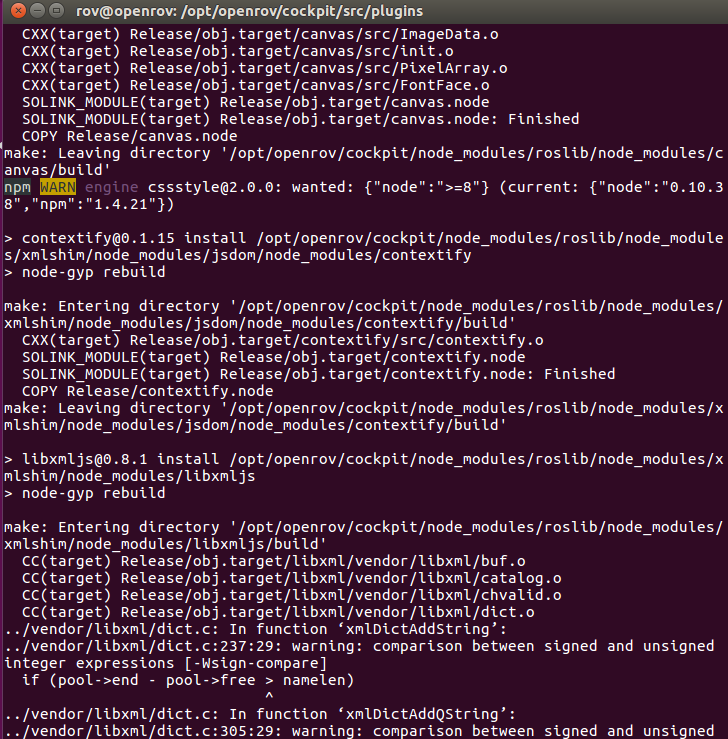
\includegraphics[scale=0.70]{partes/ImgSophia/ApendiceB/instalacionRoslib2.png}
            \caption{Error durante la instalación de una de las dependencias de roslib}
            \label{fig:InsRoslib2}
        \end{figure}

\subsubsection{Instalación del plugin ros}
\begin{verbatim}
$ git clone https://github.com/sophiafakih/plugin-roslibjs.git ros    
\end{verbatim}

Si llegase a aparecer un error: \verb|the requested URL returned error: 400|, la solución es escribir manualmente la línea, porque al hacer "copiar+pegar" en el terminal pueden aparecer algunos caracteres invisibles Unicode que corrompen la instalación.

\subsubsection{Modificaciones finales}
\par Luego de haber realizado todas las descargas necesarias de internet es importante modificar de nuevo la interfaz eth0 en \verb|/etc/network/interfaces| y descomentar la IP estática: 192.168.254.1 con sus demás parámetros, para que ese archivo regrese a la forma por defecto en la que permite visualizar el cockpit en dicha IP. 

\par Posteriormente, desde el Cloud9 o mediante la conexión SSH se tiene que buscar el archivo que dió error durante la instalación \ref{fig:InsRoslib2} y eliminar su contenido. Sin embargo, vale la pena recalcar que el error presentado se encontraba en la línea 10, basicamente por problemas de compatibilidad con la versión node.js que se ejecuta en el OpenROV.

\begin{verbatim}
$ sudo nano /opt/openrov/cockpit/src/node_modules/roslib/node_modules
/xmlshim/node_modules/jsdom/node_modules/cssstyle/lib
/CSSStyleDeclaration.js
\end{verbatim}

        \begin{figure}[H]
            \centering
            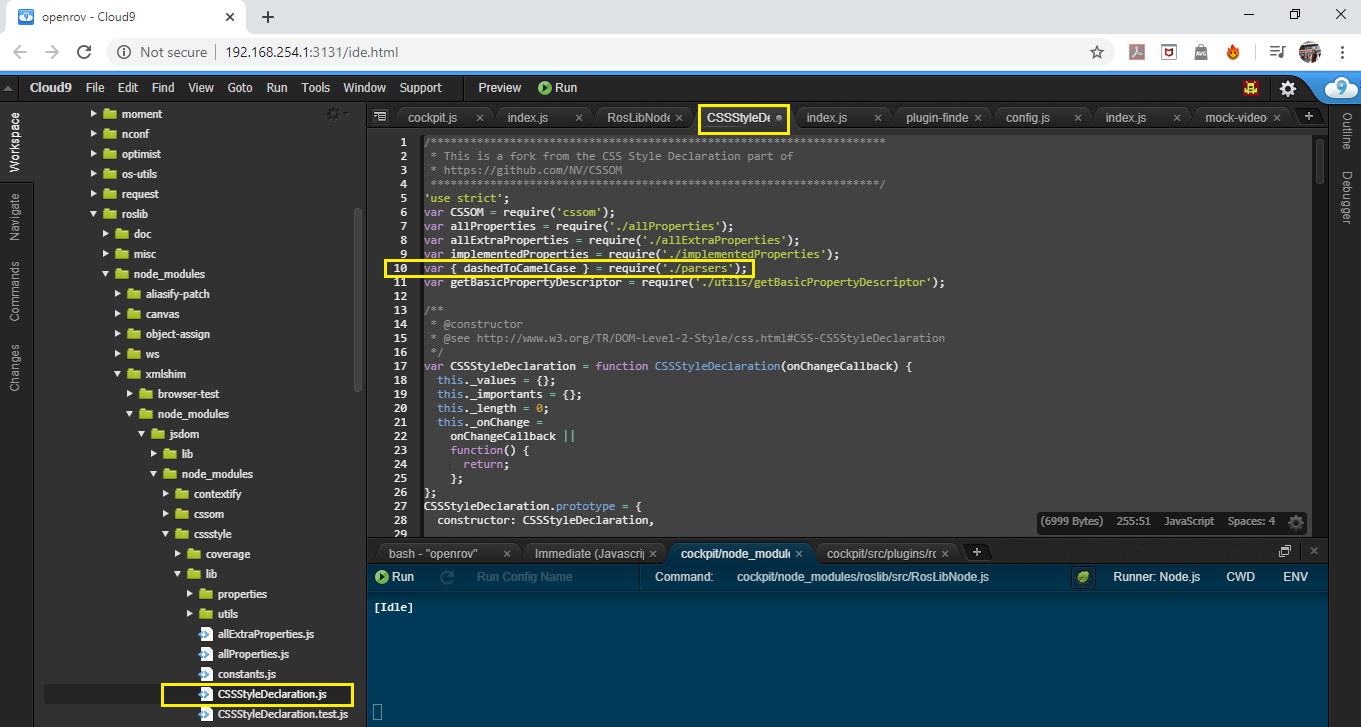
\includegraphics[scale=0.40]{partes/ImgSophia/ApendiceB/ArchivoAEliminar.png}
            \caption{Archivo a eliminar por corromper la instalación de roslib}
            \label{fig:FileToDelete}
        \end{figure}

\par Mientras el contenido de este archivo se encuentre presente, se obtiene un error al tratar de abrir el cockpit (no carga), dado que existen bugs dentro del proceso Node.js: en el index.js del plugin ros no se realiza el require=(``roslib") de la línea 5, por errores de compilación en el archivo principal de esa librería. 

\section{Instalaciones en la computadora: ROS}

La interfaz fue probada usando Ubuntu 16.04 con ROS Kinetic Kame.

    \subsection{Instalación de ROS desktop full}

    \begin{verbatim}
	$ sudo sh -c 'echo "deb http://packages.ros.org/ros/ubuntu 
	`lsb_release -sc` main" > /etc/apt/sources.list.d/ros-latest.list'
	
	$ sudo apt-get update
	
	$ sudo apt-get install ros-kinetic-desktop-full
	
	$ sudo rosdep init
	$ rosdep update
	
	$ echo "source ~/catkin_ws/devel/setup.bash" >> ~/.bashrc
	$ source ~/.bashrc
	
	$ sudo apt install python-rosinstall python-rosinstall-generator 
	python-wstool build-essential
	\end{verbatim}
	
    \subsection{Creación del espacio de trabajo en ROS}
	
	\begin{verbatim}
	$ mkdir -p ~/catkin_ws/src
$ cd ~/catkin_ws/
	$ catkin_make
    \end{verbatim}
	
    \subsection{Instalación Rosbridge}
    \begin{verbatim}
$ sudo apt-get install ros-kinetic-rosbridge-server
$ sudo apt-get install ros-kinetic-rosbridge-suite
$ source /opt/ros/kinetic/setup.bash
    \end{verbatim}
    
    \subsection{Instalación gscam}
    \begin{verbatim}
$ sudo apt-get update && sudo apt-get install gstreamer0.10 
gstreamer0.10-plugins-base gstreamer0.10-plugins-base-apps 
gstreamer0.10-plugins-good libgstreamer0.10-dev 
libgstreamer-plugins-base0.10-dev

$ sudo apt-get install ros-kinetic-rqt 
ros-kinetic-camera-calibration-parsers 
ros-kinetic-camera-info-manager ros-kinetic-cv-bridge 
ros-kinetic-image-transport

$ cd ~/catkin_ws/src
$ git clone https://github.com/ros-drivers/gscam.git
$ cd ~/catkin_ws/
$ catkin_make
    \end{verbatim}
    
    
    \subsection{Instalación del paquete OpenROV-ros}

	\begin{verbatim}
	$ cd ~/catkin_ws/src
$ git clone https://github.com/sophiafakih/OpenROV-ros.git openrov
$ cd ~/catkin_ws/
$ catkin_make
	$ echo "source ~/catkin_ws/devel/setup.bash" >> ~/.bashrc
	$ source ~/.bashrc
	\end{verbatim}



	






